\chapter{フィードバック変調器}
\label{sec:FBM}
本章では,\ref{sec:IntegrationControl}章のコンプライアンス制御において使用したフィードバック変調器(Feedback Module:FBM)について述べる.
FBMは石川らにより提案された離散値入力制御器の一つであり,フィードバック構造を持つことで量子化における誤差を低減が可能である\cite{石川将人2007,石川将人2008フィードバック変調器を用いた離散値入力制御におけるアクチュエータ非線形性の補償}.
また,同様にフィードバック構造を持つ$\Delta\Sigma$変調器と比べて,切り替え時間の遅いアクチュエータでも有効であること,離散値入力システムに対し連続値入力システムとして制御設計ができることが利点である.
その構造を\figname\ref{fig:FBM}に示す.
S/Hはサンプリング時間$h$のサンプラーとゼロ次ホルダーであり,時間分解能制約を表す.
Quantizerは量子化器であり,空間分解能制約を表す.
また,$Q(s)$は設計パラメータであり,
\begin{align}
    \label{eq:FBM_Qs}
    Q(s)\in RH_\infty,~~Q(\infty) = 0
\end{align}
を満たす.
$u$がFBMに対する入力,$u_Q$が出力であり,$u_C$はS/Hへの入力である.

\begin{figure}[t]
    \centering
        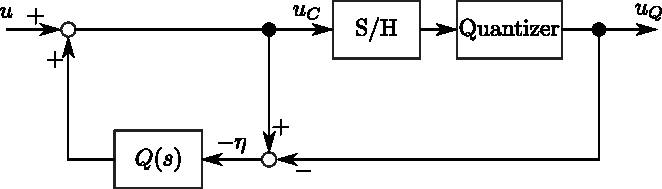
\includegraphics[keepaspectratio, scale=1.0]{contents/Appendix_FBM/figure/FBM.pdf}
        \caption{Structure of FBM}
        \label{fig:FBM}
\end{figure}

$\eta$はS/Hおよび量子化器により発生する誤差であり,
\begin{align}
    \label{eq:FBM_eta}
    \eta = u_Q-u_C
\end{align}
となる.
また,FBMの入出力関係は
\begin{align}
    \label{eq:FBM_IO}
    u_Q = u + {1-Q(s)}\eta
\end{align}
表せ,パラメータ$N(s)$を
\begin{align}
    \label{eq:FBM_Ns}
    N(s) := 1-Q(s)
\end{align}
と定義すると,これは$\eta$から$u_Q$への伝達関数\footnote{雑音伝達関数(Noise transfer function: NTF)と呼ばれる.}であり,誤差$\eta$は$N(s)$で周波数整形される.
$Q(s)=0$のときがフィードバックのない通常の量子化器になる.

ここで,$N(s)$を
\begin{align}
    \label{eq:FBM_Ns2}
    N(s) = \left(\frac{\tau s}{\tau s + 1} \right)^2
\end{align}
と定めると,$h<\tau$を満たすとき,FBMはBIBO安定となる.

本研究においては,$h=0.02$,$\tau=0.022$とした.